\documentclass[a4paper,11pt]{report}
\usepackage[showexo=true,showcorr=false]{../packages/coursclasse}

%Commenter ou enlever le commentaire sur la ligne suivante pour montrer le niveau
\toggletrue{montrerNiveaux}
%permet de gérer l'espacement entre les items des env enumerate et enumitem

\usepackage{enumitem}
\setlist[enumerate]{align=left,leftmargin=1cm,itemsep=5pt,parsep=0pt,topsep=0pt,rightmargin=0.5cm}
\setlist[itemize]{align=left,labelsep=1em,leftmargin=*,itemsep=0pt,parsep=0pt,topsep=0pt,rightmargin=0cm}
%permet de gerer l'espacement entre les colonnes de multicols
\setlength\columnsep{20pt}


\begin{document}
%%%%%%%%%%%%%%%%% À MODIFIER POUR CHAQUE SERIE %%%%%%%%%%%%%%%%%%%%%%%%%%%%%
\newcommand{\chapterName}{Espace}
\newcommand{\serieName}{Reconnaissance, dénomination \\ et description de solides}


%%%%%%%%%%%%%%%%%% PREMIERE PAGE NE PAS MODIFER %%%%%%%%%%%%%%%%%%%%%%%%
% le chapitre en cours, ne pas changer au cours d'une série
\chapter*{\chapterName}
\thispagestyle{empty}

%%%%% LISTE AIDE MEMOIRE %%%%%%
\begin{amL}{\serieName}{
\item Polyèdre (page 144)
\item Prisme droit (page 145)
\item Parallélépipède rectange ou pavé droit (page 146)}
\end{amL}
%%%%%%%%%%%%%%% DEBUT DE LA SERIE NE PAS MODIFIER %%%%%%%%%%%%%%%%%%%%%%%%%%%%%
\section*{\serieName}
\setcounter{page}{1}
\thispagestyle{firstPage}



%%%%%%%%%%% LES EXERCICES %%%%%%%%%%%%%%%%%%%%%%%%%%%%%%%%%%%

\begin{exop}{
Détermine le nombre de faces, d'arêtes et de sommets dans les solides suivants.	
\begin{tasks}[after-item-skip = 0.4em](3)
	\task 

	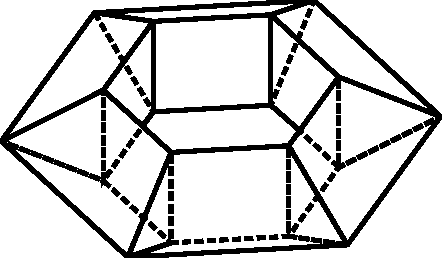
\includegraphics[scale=0.5]{media/es-21/tp1}
	\task 

	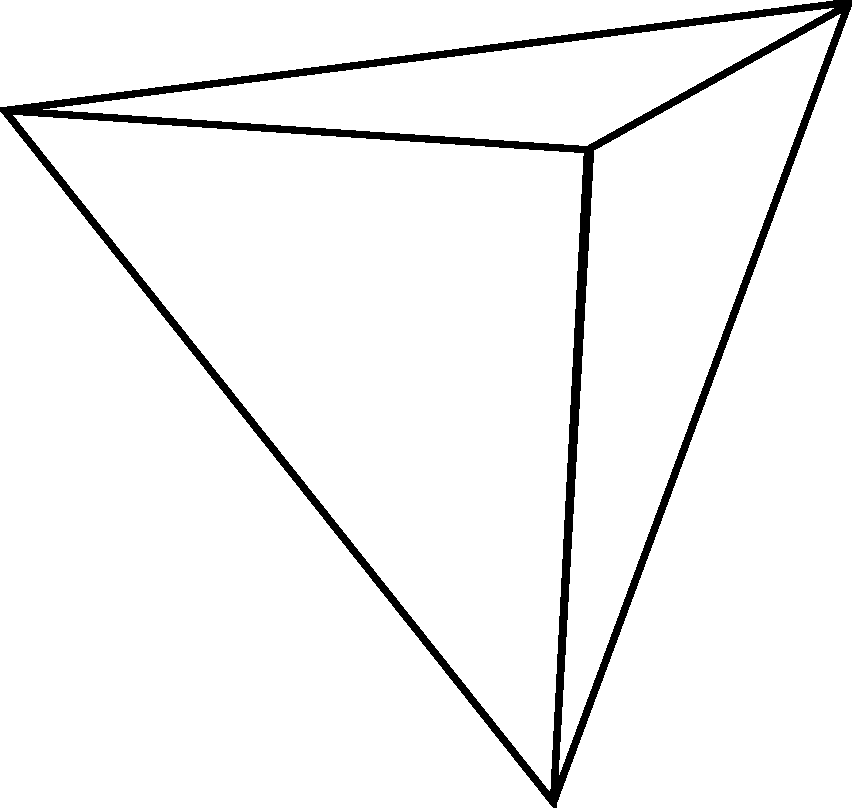
\includegraphics[scale=0.25]{media/es-21/tp2}
	\task 

	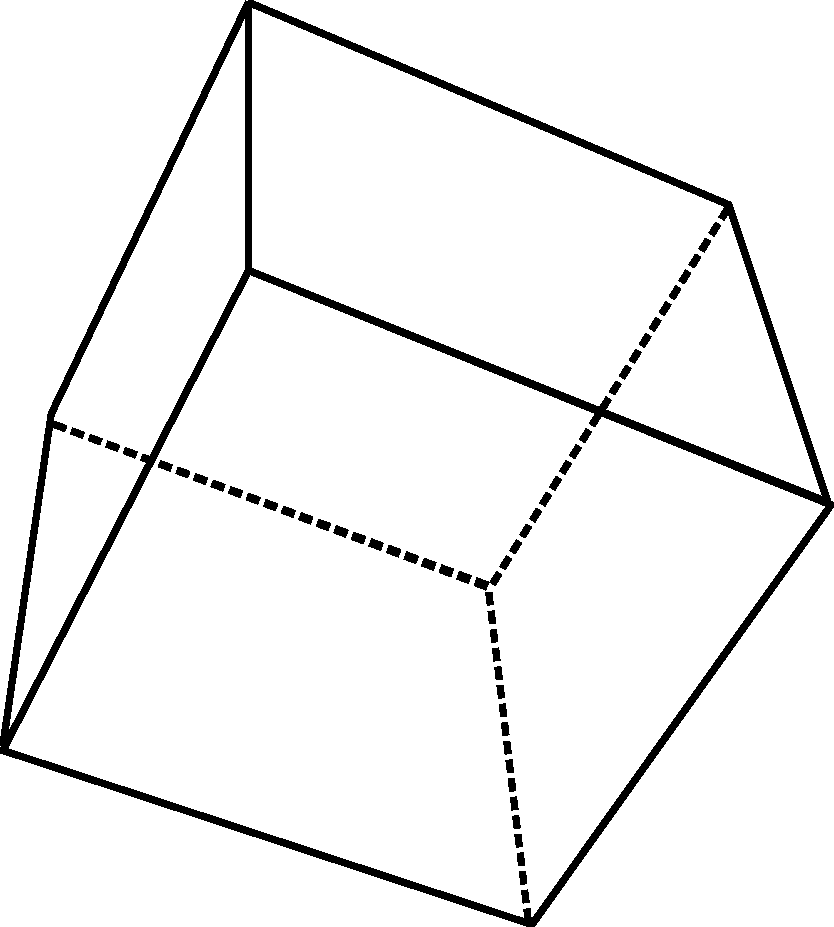
\includegraphics[scale=0.25]{media/es-21/tp3}
	\vspace{-2cm}
	\task 

	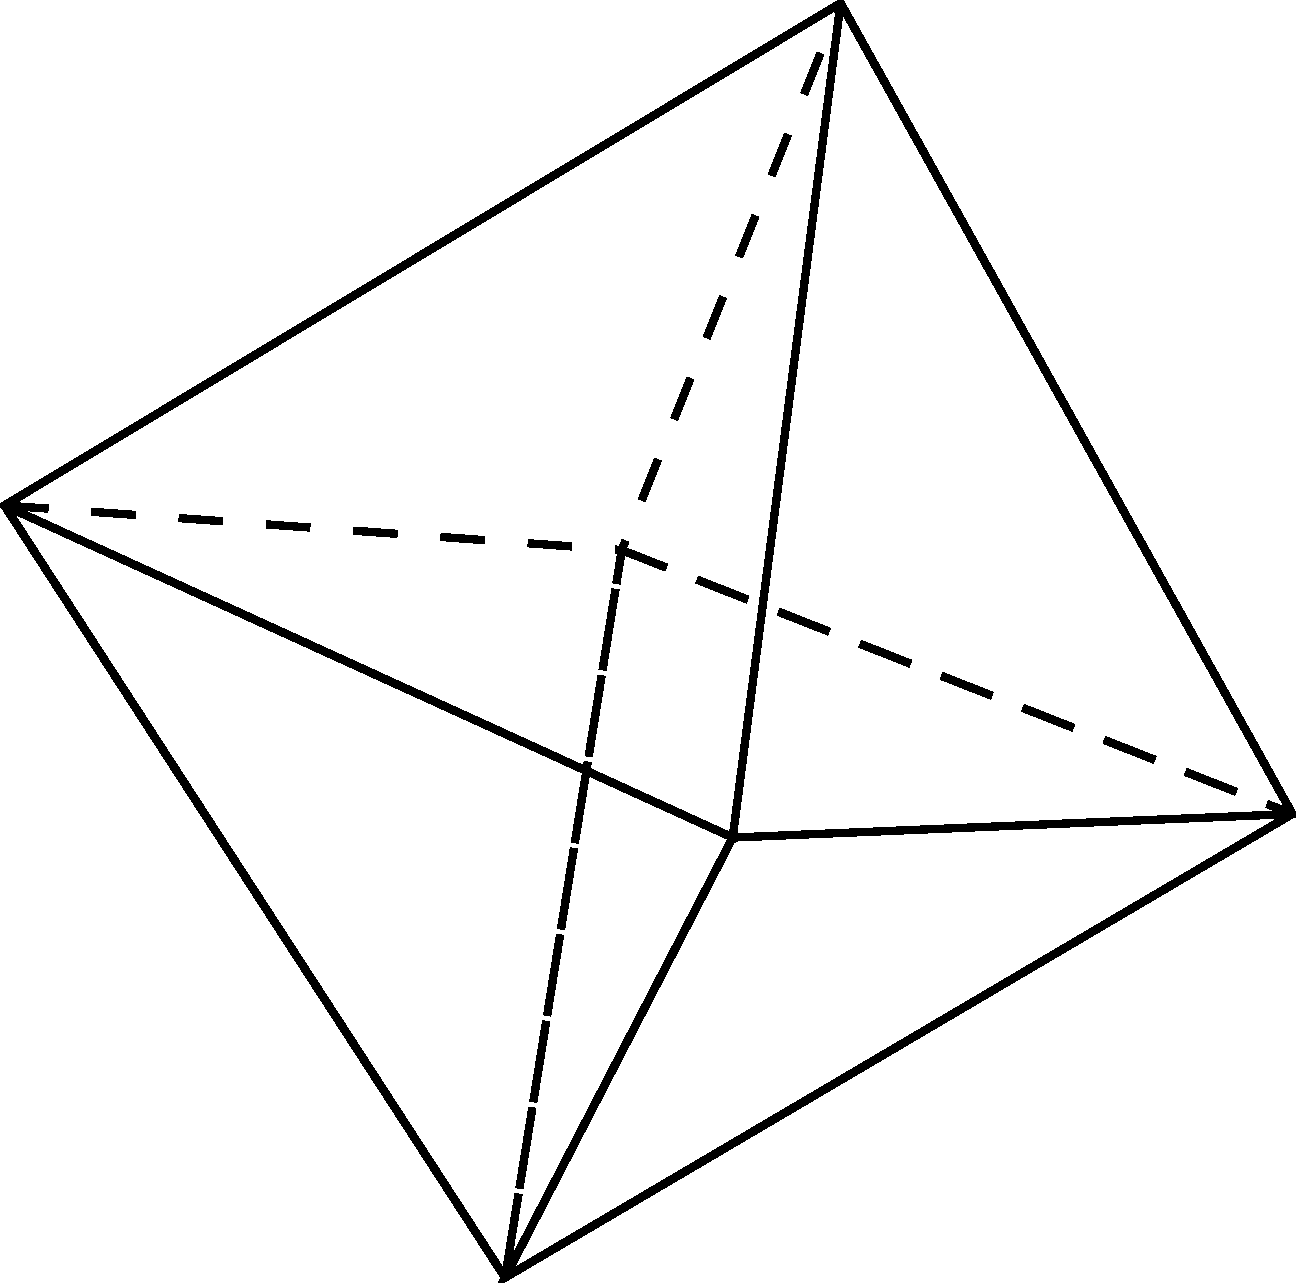
\includegraphics[scale=0.17]{media/es-21/tp4}
	\task 

	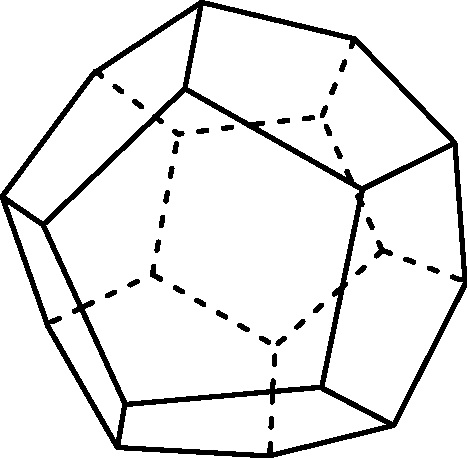
\includegraphics[scale=0.4]{media/es-21/tp5}
\end{tasks}
	}{1}
\end{exop}
\begin{exop}{
Détermine le nombre de faces, d'arêtes et de sommets dans les solides suivants.	
\begin{tasks}(4)
	\task 

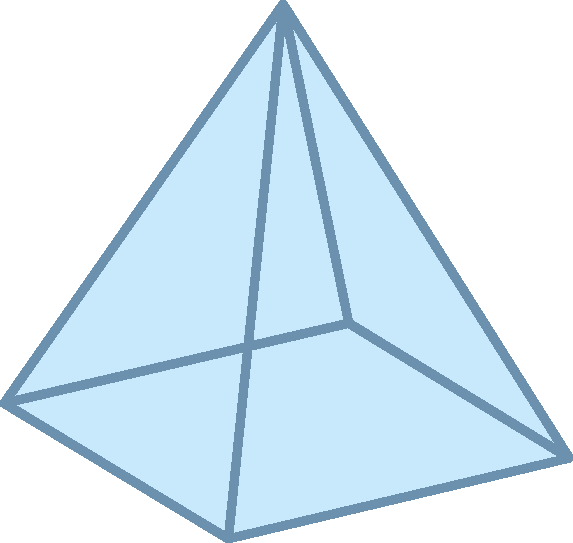
\includegraphics[scale=0.3]{media/es-21/pyra_blue}
\task

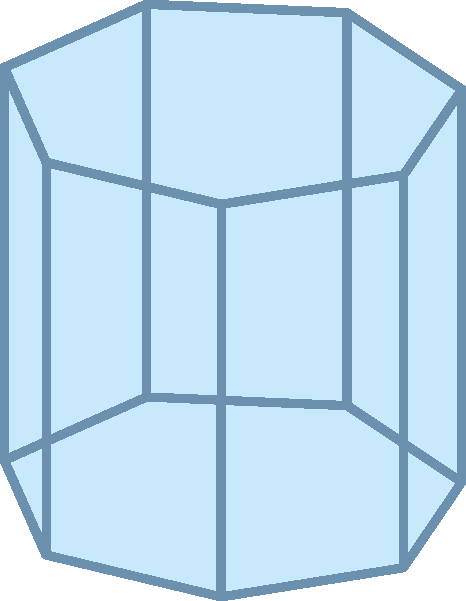
\includegraphics[scale=0.3]{media/es-21/prism_hexa_blue}
\task

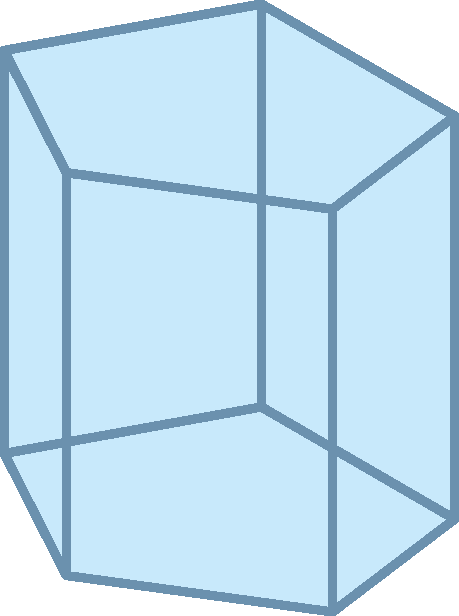
\includegraphics[scale=0.3]{media/es-21/prism_penta_blue}
\task


\includegraphics[scale=0.3]{media/es-21/prism_triang_blue}
\end{tasks}
}{1}
\end{exop}
\begin{exol}{ES99}{118}{1}
\end{exol}
\begin{exop}{
Parmi les solides suivants, lesquels sont des prismes droits? Si ce sont des prismes droits:
\begin{itemize}
	\item Identifie les bases.
	\item Identifie une hauteur du prisme.
	\item Nomme le prisme en question.
\end{itemize}
\begin{tasks}(3)
	\task 


\includegraphics[scale=1]{media/es-21/pq1}
	\task 


\includegraphics[scale=1]{media/es-21/pq2}
	\task 

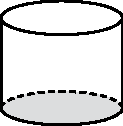
\includegraphics[scale=1]{media/es-21/pq3}
	\task 

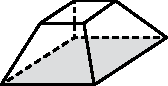
\includegraphics[scale=1]{media/es-21/pq4}
	\task 

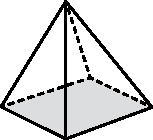
\includegraphics[scale=1]{media/es-21/pq5}
	\task 


\includegraphics[scale=1]{media/es-21/pq6}
	\task 

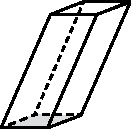
\includegraphics[scale=1]{media/es-21/pq7}
	\task 

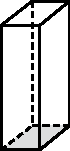
\includegraphics[scale=1]{media/es-21/pq8}
	\task 

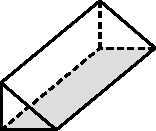
\includegraphics[scale=1]{media/es-21/pq9}
\end{tasks}
}{1}
\end{exop}
\begin{exof}{ES97}{143}{1}
\end{exof}
\begin{exof}{ES98}{144}{1}
\end{exof}
\begin{exol}{ES100}{118}{3}
\end{exol}
\end{document}

